\documentclass[svgnames,11pt]{standalone}
\usepackage[utf8]{inputenc}
\usepackage[T1]{fontenc}
\usepackage{csquotes}
\usepackage[english]{babel}
\usepackage{xcolor}
\usepackage{charter}
\usepackage{amsmath}
\usepackage{amssymb}
\usepackage[np,autolanguage]{numprint}
\newcommand{\outqt}[1]{{\textcolor{DarkOrange}{#1}}}
\newcommand{\inqt}[1]{{\textcolor{Blue}{#1}}}
\usepackage{tikz}
\usetikzlibrary{arrows,automata,calc}
\usetikzlibrary{arrows.meta}
\usetikzlibrary{decorations.pathreplacing}
\usetikzlibrary{backgrounds,shapes}
\tikzset{%
  show curve controls/.style={
    postaction={
      decoration={
        show path construction,
        curveto code={
          \draw [blue] 
            (\tikzinputsegmentfirst) -- (\tikzinputsegmentsupporta)
            (\tikzinputsegmentlast) -- (\tikzinputsegmentsupportb);
          \fill [red, opacity=0.5] 
            (\tikzinputsegmentsupporta) circle [radius=.25ex]
            (\tikzinputsegmentsupportb) circle [radius=.25ex];
        }
      },
      decorate
}}}
\tikzstyle{vertex}=[draw,circle,black,inner sep=2pt]
\tikzstyle{edge}=[line width=1.3pt,color=Black]
\tikzstyle{rare}=[fill=black,text=white]
\tikzstyle{medium}=[fill=black!15!white]


\begin{document}
  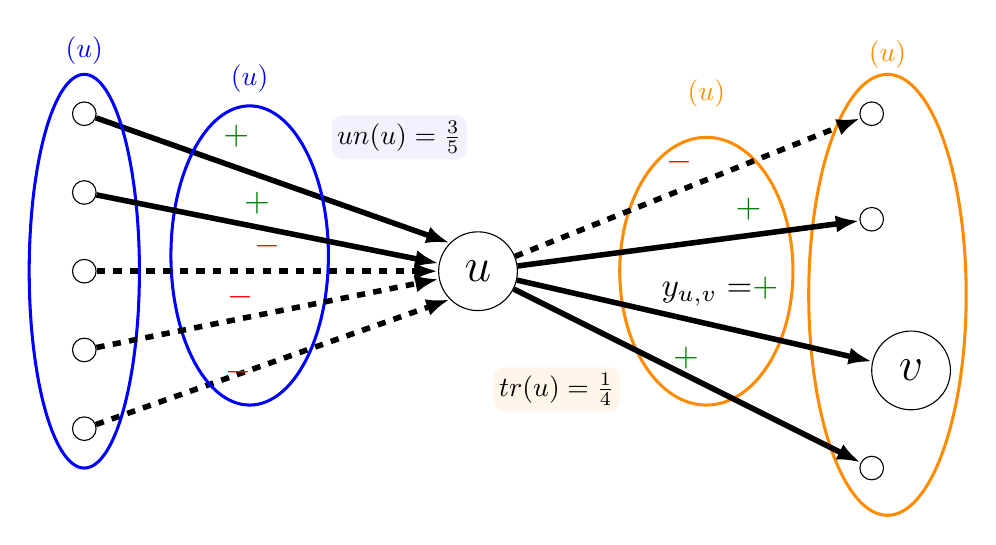
\begin{tikzpicture}[auto,vertex/.append style={minimum width=10mm,font=\Large,fill=White},
        scale=1.0,]
      \tikzset{>=latex}
      \tikzstyle{edge}=[line width=2pt,color=Black,-{Latex[length=3mm,width=1.0mm,angle'=40]}]
      \tikzstyle{trainEdge}=[line width=10pt,color=Black!15,opacity=0]
      \tikzstyle{elabel}=[color=Black]
      \tikzstyle{holder}=[draw,circle,black,inner sep=1pt, minimum width=3mm]
      \tikzstyle{posc}=[scale=1.2,text=Green]
      \tikzstyle{negc}=[scale=1.2,text=red]
      \tikzstyle{testset}=[opacity=1.0]
      \tikzstyle{revealed}=[circle,draw=none,fill=none,inner sep=1pt,]

      \draw[DarkOrange,line width=1.1pt] (5.2, -0.3) ellipse [x radius=1,y radius=2.8] node[yshift=3.05cm] {$\NNout(u)$};
      \draw[DarkOrange,line width=1.1pt] (2.9, 0) ellipse [x radius=1.1,y radius=1.7] node[yshift=2.25cm] {$\Nout(u)$};
      \draw[Blue,line width=1.1pt] (-5, 0) ellipse [x radius=0.7,y radius=2.5] node[yshift=2.8cm] {$\NNin(u)$};
      \draw[Blue,line width=1.1pt] (-2.9, 0.2) ellipse [x radius=1,y radius=1.9] node[yshift=2.25cm] {$\Nin(u)$};
      \node[vertex] (u) at (0,0) {\LARGE $u$};
      \node[vertex] (v) at (5.5,-1.26) {\LARGE $v$};

      \node[holder] (fromu1) at (5, -2.5) {};
      % \draw[trainEdge] (u) --                                                       (5, -2.5);
      \draw[edge] (u) -- node [revealed,posc,xshift=-2mm,] {$\mathbf{+}$}           (fromu1);

      \draw[testset,edge] (u) edge  node [posc,xshift=-5mm]
        {${\textcolor{Black}{y_{u,v}=}}{\textcolor{Green}{+}}$} (v);
      \node[holder] (fromu2) at (5, .66) {};
      \node[holder] (fromu3) at (5, 2) {};
      \draw[testset,edge] (u) edge  node [posc,xshift=2mm,pos=0.7] {$\mathbf{+}$}            (fromu2);
      \draw[testset,edge, dashed] (u)   edge   node [negc,xshift=2mm] {$\mathbf{-}$} (fromu3);

      \node[holder] (tou1) at (-5, -2) {};
      \node[holder] (tou2) at (-5, -1) {};
      \node[holder] (tou3) at (-5, 0) {};
      \node[holder] (tou4) at (-5, 1) {};
      \node[holder] (tou5) at (-5, 2) {};
      \begin{scope}[on background layer]
        % \draw[trainEdge] (-5, -2) --    (u.south west);
        \draw[edge, dashed] (tou1)       -- node[revealed,negc,yshift=-3mm,xshift=-5pt] {$\mathbf{-}$} (u.south west);
        % \draw[trainEdge,]          (-5, 2) -- (u.north west);
        \draw[edge,]               (tou5) -- node[revealed,posc,above,pos=0.35,xshift=5pt] {$\mathbf{+}$} (u.north west);
      \end{scope}

      \draw[testset,edge,dashed] (tou2)-- node[negc,yshift=-1mm] {$\mathbf{-}$} (u);
      \draw[testset,edge,dashed] (tou3) -- node[negc] {$\mathbf{-}$} (u);
      \draw[testset,edge,]       (tou4) -- node[posc,xshift=-4mm] {$\mathbf{+}$} (u);


      \node[fill=white!90!DarkOrange,fill opacity=.9,text opacity=1,rounded corners,inner sep=2pt] at (1,-1.5) {$tr(u)=\frac{1}{4}$};
      \node[fill=white!90!Blue,fill opacity=.5,text opacity=1,rounded corners,inner sep=2pt] at (-1.0,1.7) {$un(u)=\frac{3}{5}$};
\end{tikzpicture}
\end{document}
